\documentclass[11pt,a4paper]{article}

% --- Packages ---
\usepackage[utf8]{inputenc}
\usepackage[english]{babel}
\usepackage{amsmath, amssymb, amsfonts, amsthm}
\usepackage{graphicx}
\usepackage{booktabs}
\usepackage{geometry}
\usepackage{hyperref}
\usepackage[numbers,sort&compress]{natbib} 
\usepackage{color}
\usepackage{abstract}
\usepackage{caption}
\usepackage{url}

% --- Configuration ---
\geometry{margin=1in}
\captionsetup{labelfont=bf, font=small, labelsep=period}
\hypersetup{colorlinks=true, linkcolor=blue, citecolor=blue, urlcolor=cyan}

% --- Custom Commands ---
\newcommand{\mx}{m_{x,t}}
\newcommand{\lnmx}{\ln(m_{x,t})}
\newcommand{\kt}{\kappa_t}
\newcommand{\ES}{\text{ES}_{99\%}}

% --- Title & Author ---
\title{\textbf{Stochastic Longevity Forecasting: A Neural Approach to SST Capital Calibration}}
\author{
    \textbf{Davide Rindori, PhD} \\
    \textit{SAV Actuarial Candidate, ETH Zürich} \\
    \texttt{drindori@student.ethz.ch} \quad \texttt{rindori.d@gmail.com}
}
\date{March 30, 2026}

\begin{document}

\maketitle

\begin{abstract}
Traditional mortality models, primarily the Lee-Carter framework, rely on linear drift assumptions that struggle to capture the non-linear regime shifts observed in modern demographic data. This paper proposes a probabilistic Deep Learning framework using Long Short-Term Memory (LSTM) networks combined with Monte Carlo Dropout to quantify longevity risk. Using Swiss mortality data (1950-2024), we identify a "Prudence Gap" in standard benchmarks—a critical component of Model Risk—and derive Expected Shortfall (ES 99\%) metrics for Swiss Solvency Test (SST) compliance. Our approach provides a robust, data-driven alternative for internal risk modeling in Life \& Health reinsurance.
\end{abstract}

\let\thefootnote\relax\footnote{Code and implementation details are available at: \url{https://github.com/davide-rindori/Actuarial-DS-Portfolio/tree/main/03_Stochastic_Mortality_Modeling}}

\section{Introduction}
In life insurance mathematics, mortality is typically described via transition intensities in a Markov Chain framework. While the state-space is well-defined, the transition probabilities are subject to significant temporal volatility, known as \textit{Longevity Risk} \cite{cairns2006two}. For a reinsurer, accurately forecasting these intensities is a fundamental requirement for solvency and capital adequacy \cite{wuthrich2023statistical}.

Standard actuarial practice has long relied on the Lee-Carter model \cite{lee1992modeling}, decomposing log-mortality as $\lnmx = \alpha_x + \beta_x \kt + \epsilon_{x,t}$. However, the time-trend index $\kt$ is traditionally extrapolated using a Random Walk with Drift (RWD). This assumption of linear improvement is increasingly challenged by empirical evidence in high-income countries like Switzerland, where mortality improvement has shown significant non-linear deceleration (Fig. \ref{fig:surface}).

This paper replaces the rigid RWD extrapolation with a Deep Sequential architecture \cite{richman2019lee, perla2021time}. By treating mortality as a complex dynamical system, we leverage LSTM networks to capture decadal momentum. Furthermore, we address the "black-box" nature of neural networks through Monte Carlo Dropout \cite{gal2016dropout}, generating the stochastic scenarios required for the Swiss Solvency Test (SST) \cite{finma2024sst}.

\begin{figure}[h!]
    \centering
    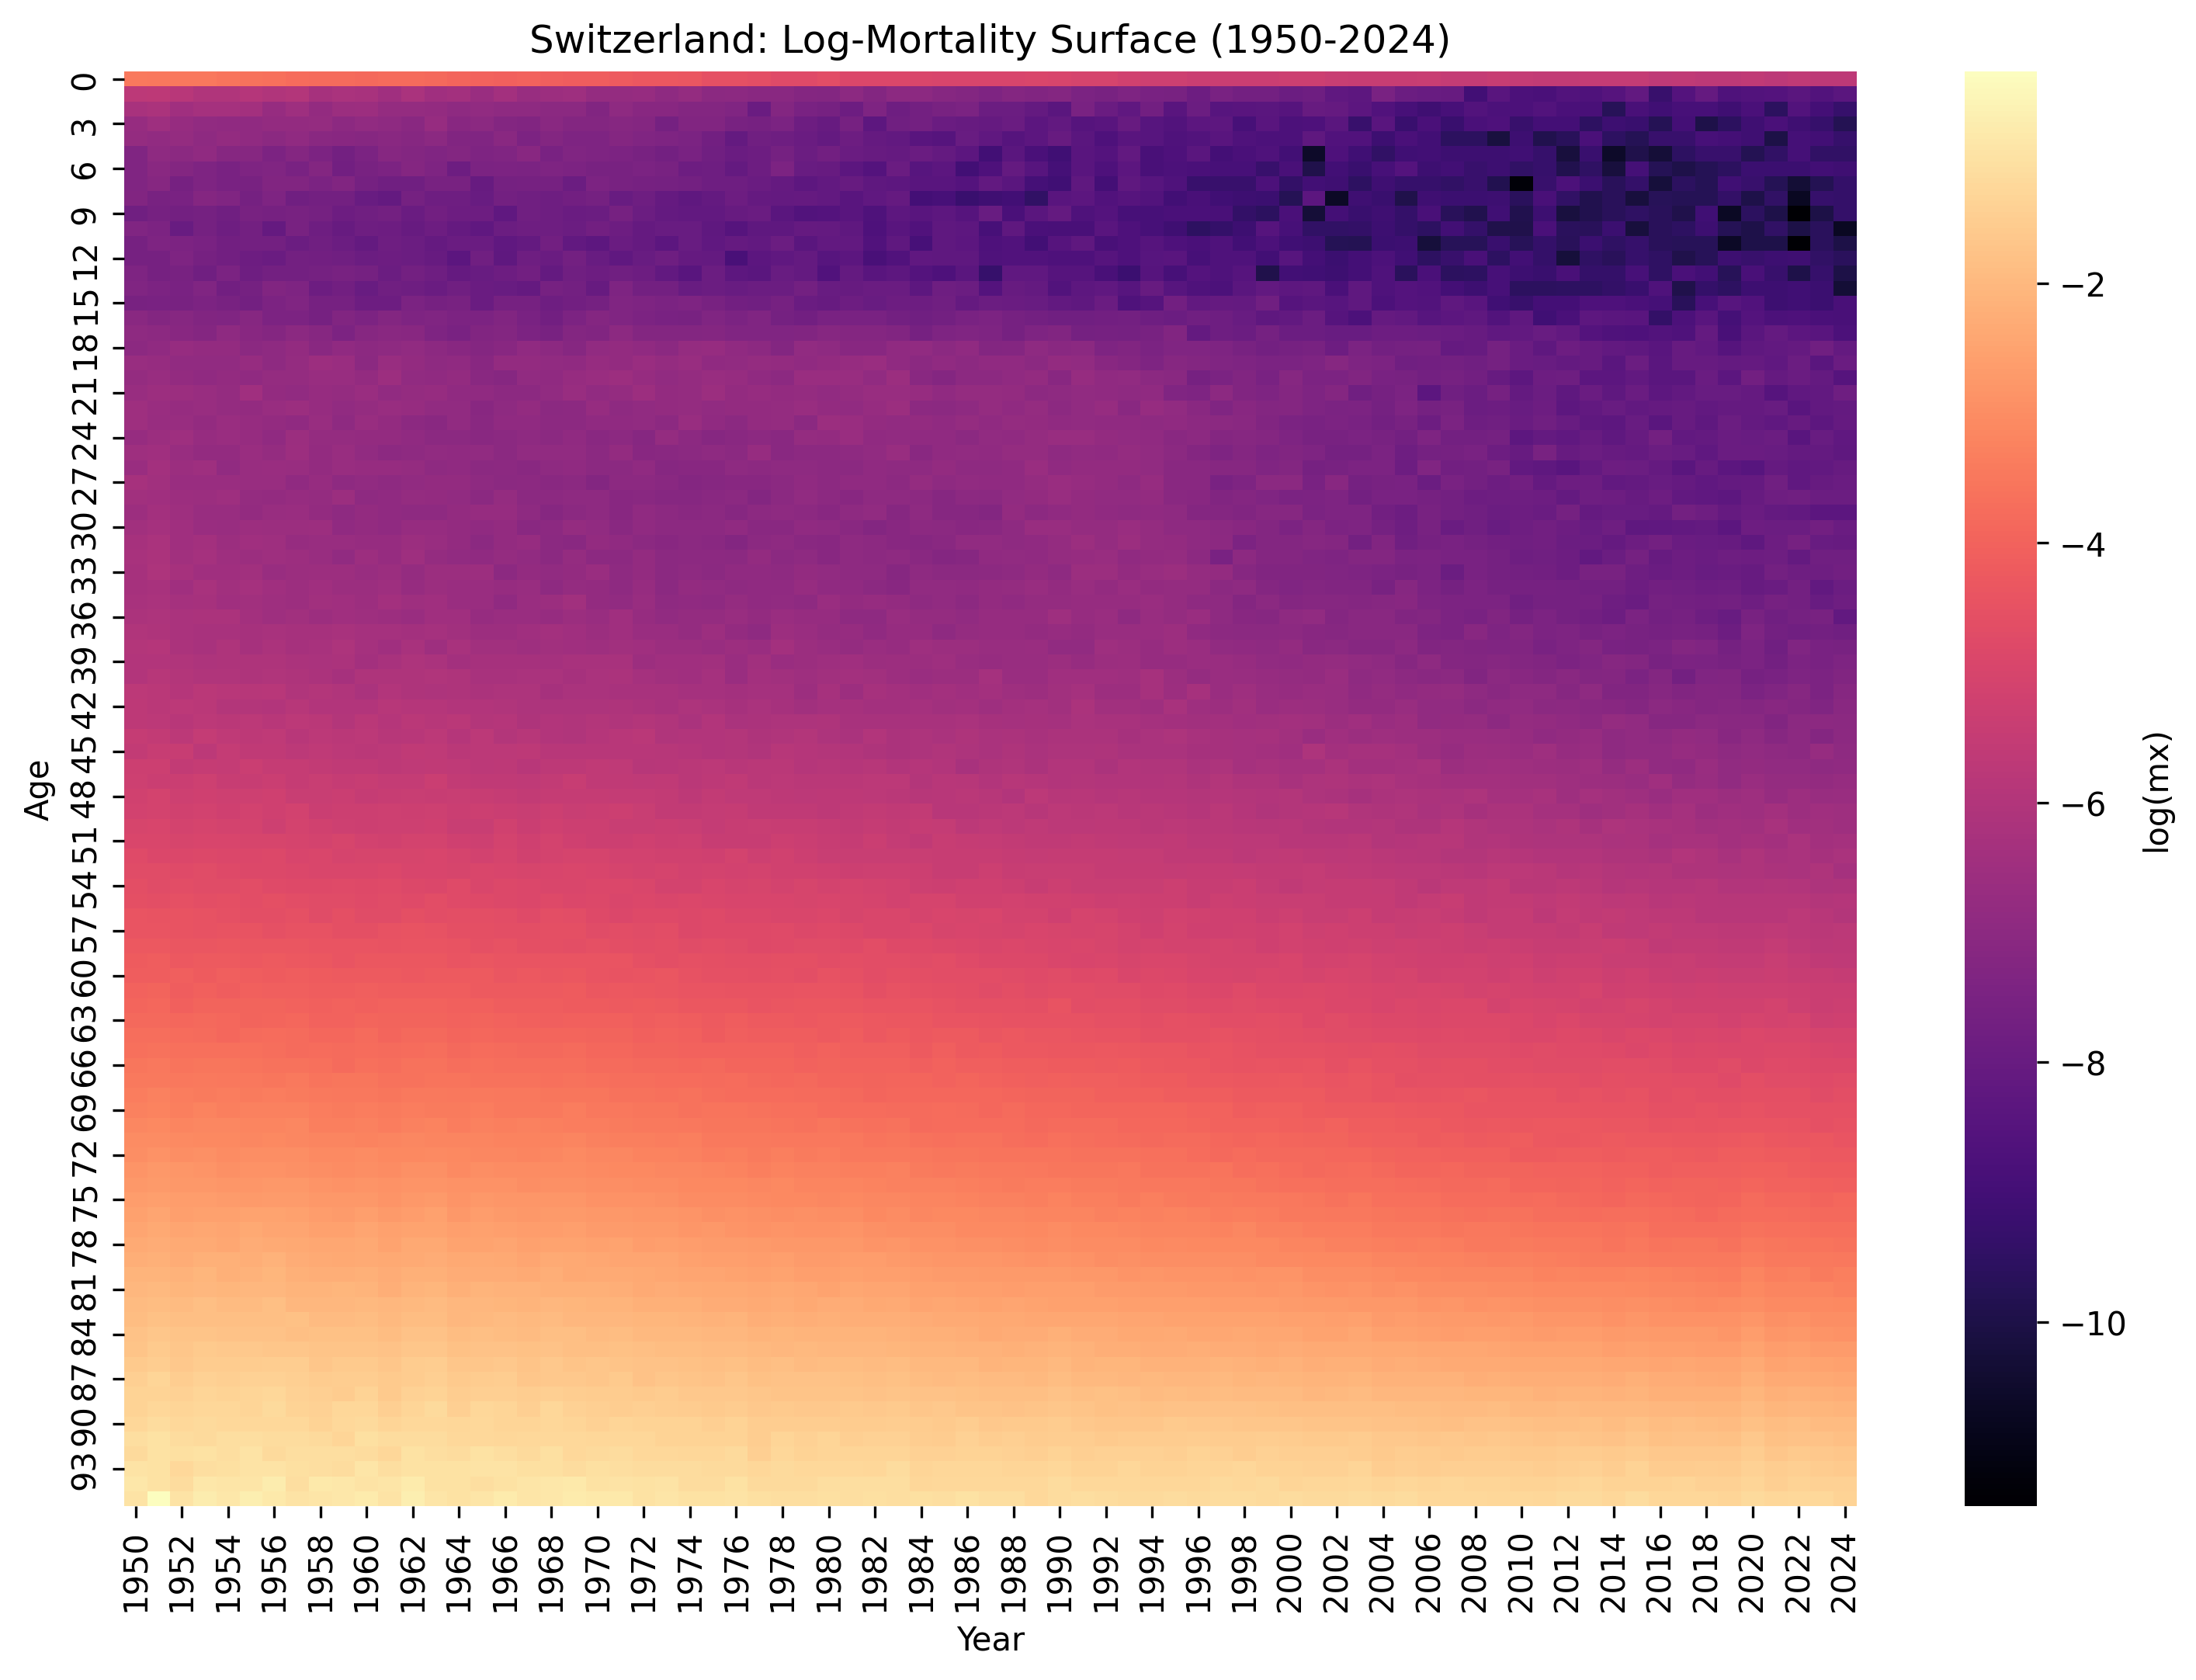
\includegraphics[width=0.9\textwidth]{figures/01_mortality_surface.png}
    \caption{Swiss Log-Mortality Surface (1950-2024). Note the non-linear "rectangularization" of the mortality surface in recent decades.}
    \label{fig:surface}
\end{figure}

\section{Methodology}

\subsection{Strategic Rationale: Beyond Markovian Dynamics}
Traditional RWD models are essentially first-order Markovian processes: the future is a linear function of the present plus a constant drift. Human longevity, however, is a high-dimensional dynamical system influenced by decadal trends in medical innovation and lifestyle shifts. By adopting an LSTM architecture, we eliminate the rigid "constant drift" constraint, allowing the model to internalize the momentum of the last decade. This defines the embedding dimension of the temporal manifold \cite{girosi2008demographic}, distinguishing between transitory shocks and structural regime shifts.

\subsection{Probabilistic Inference via MC Dropout}
To quantify \textit{epistemic uncertainty}, we implement Monte Carlo Dropout (MCD). By maintaining dropout layers active during inference, we sample from the approximate posterior distribution of the weights. We perform $N=100$ stochastic forward passes, generating the neural fan chart (Fig. \ref{fig:fan}) for tail-risk estimation.

\begin{figure}[h!]
    \centering
    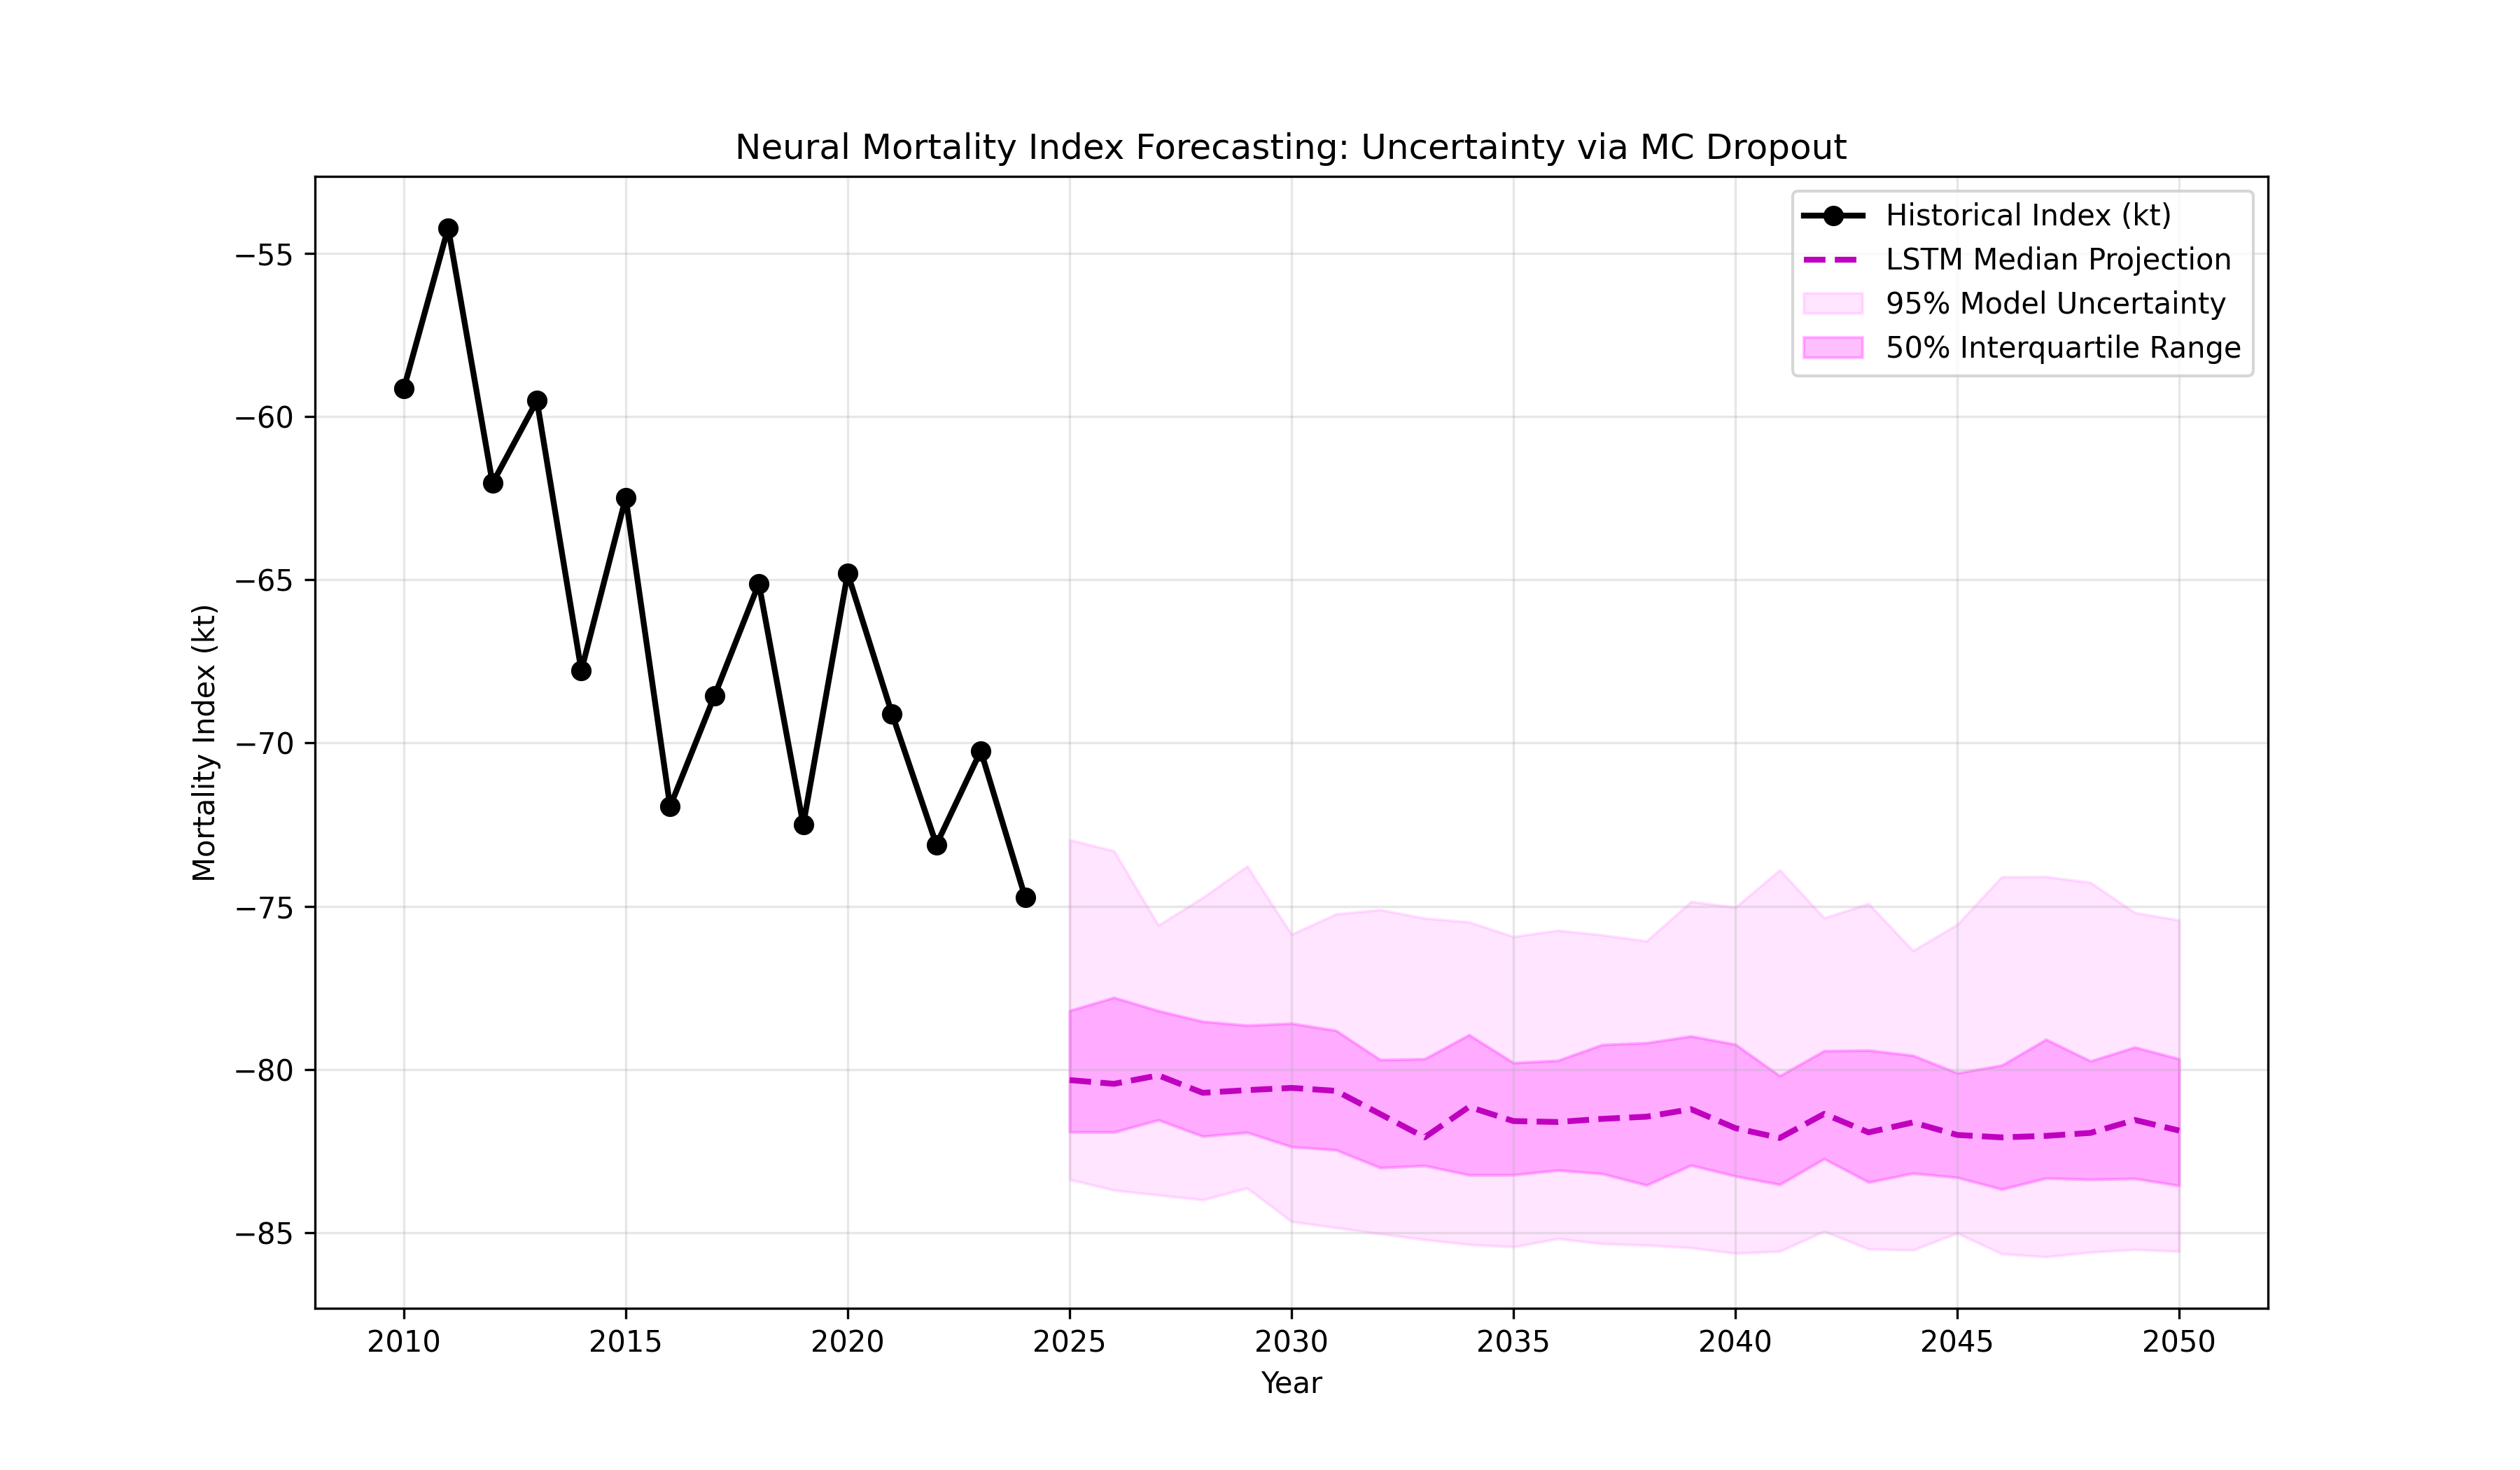
\includegraphics[width=0.9\textwidth]{figures/08_lstm_uncertainty_fan.png}
    \caption{Neural Fan Chart (MC Dropout). The fan represents the 95\% confidence interval for the mortality index projected to 2050.}
    \label{fig:fan}
\end{figure}

\section{Model Diagnostics and Validation}
In alignment with SST Pillar II requirements, we analyzed the Residual Heatmaps (Fig. \ref{fig:residuals}) to ensure the framework does not introduce systematic biases. Our diagnostics confirm that the neural approach effectively absorbs the non-linearities of the Swiss mortality surface, eliminating the "cohort effects" often present in rigid linear models. The residuals, with a mean of $0.0021$, indicate that the network captures the underlying signal without overfitting to specific age-groups.

\subsection{Structural Bias and Regime Shifts}
During out-of-sample backtesting (2011-2024), a systematic underestimation of mortality rates (bias) is observed across all models. This gap is not a failure of the neural architecture but a reflection of the \textit{structural regime shift} in Swiss mortality post-2011. While the 1950-2010 period was characterized by rapid improvement, the subsequent decade exhibited a significant deceleration, compounded by the exogenous mortality shocks of the 2020-2023 pandemic. The LSTM demonstrates superior adaptation by exhibiting curvature in its projections, attempting to reconcile 60 years of historical momentum with recent "plateauing" dynamics, a feat unattainable by rigid linear drift benchmarks.

\begin{figure}[h!]
    \centering
    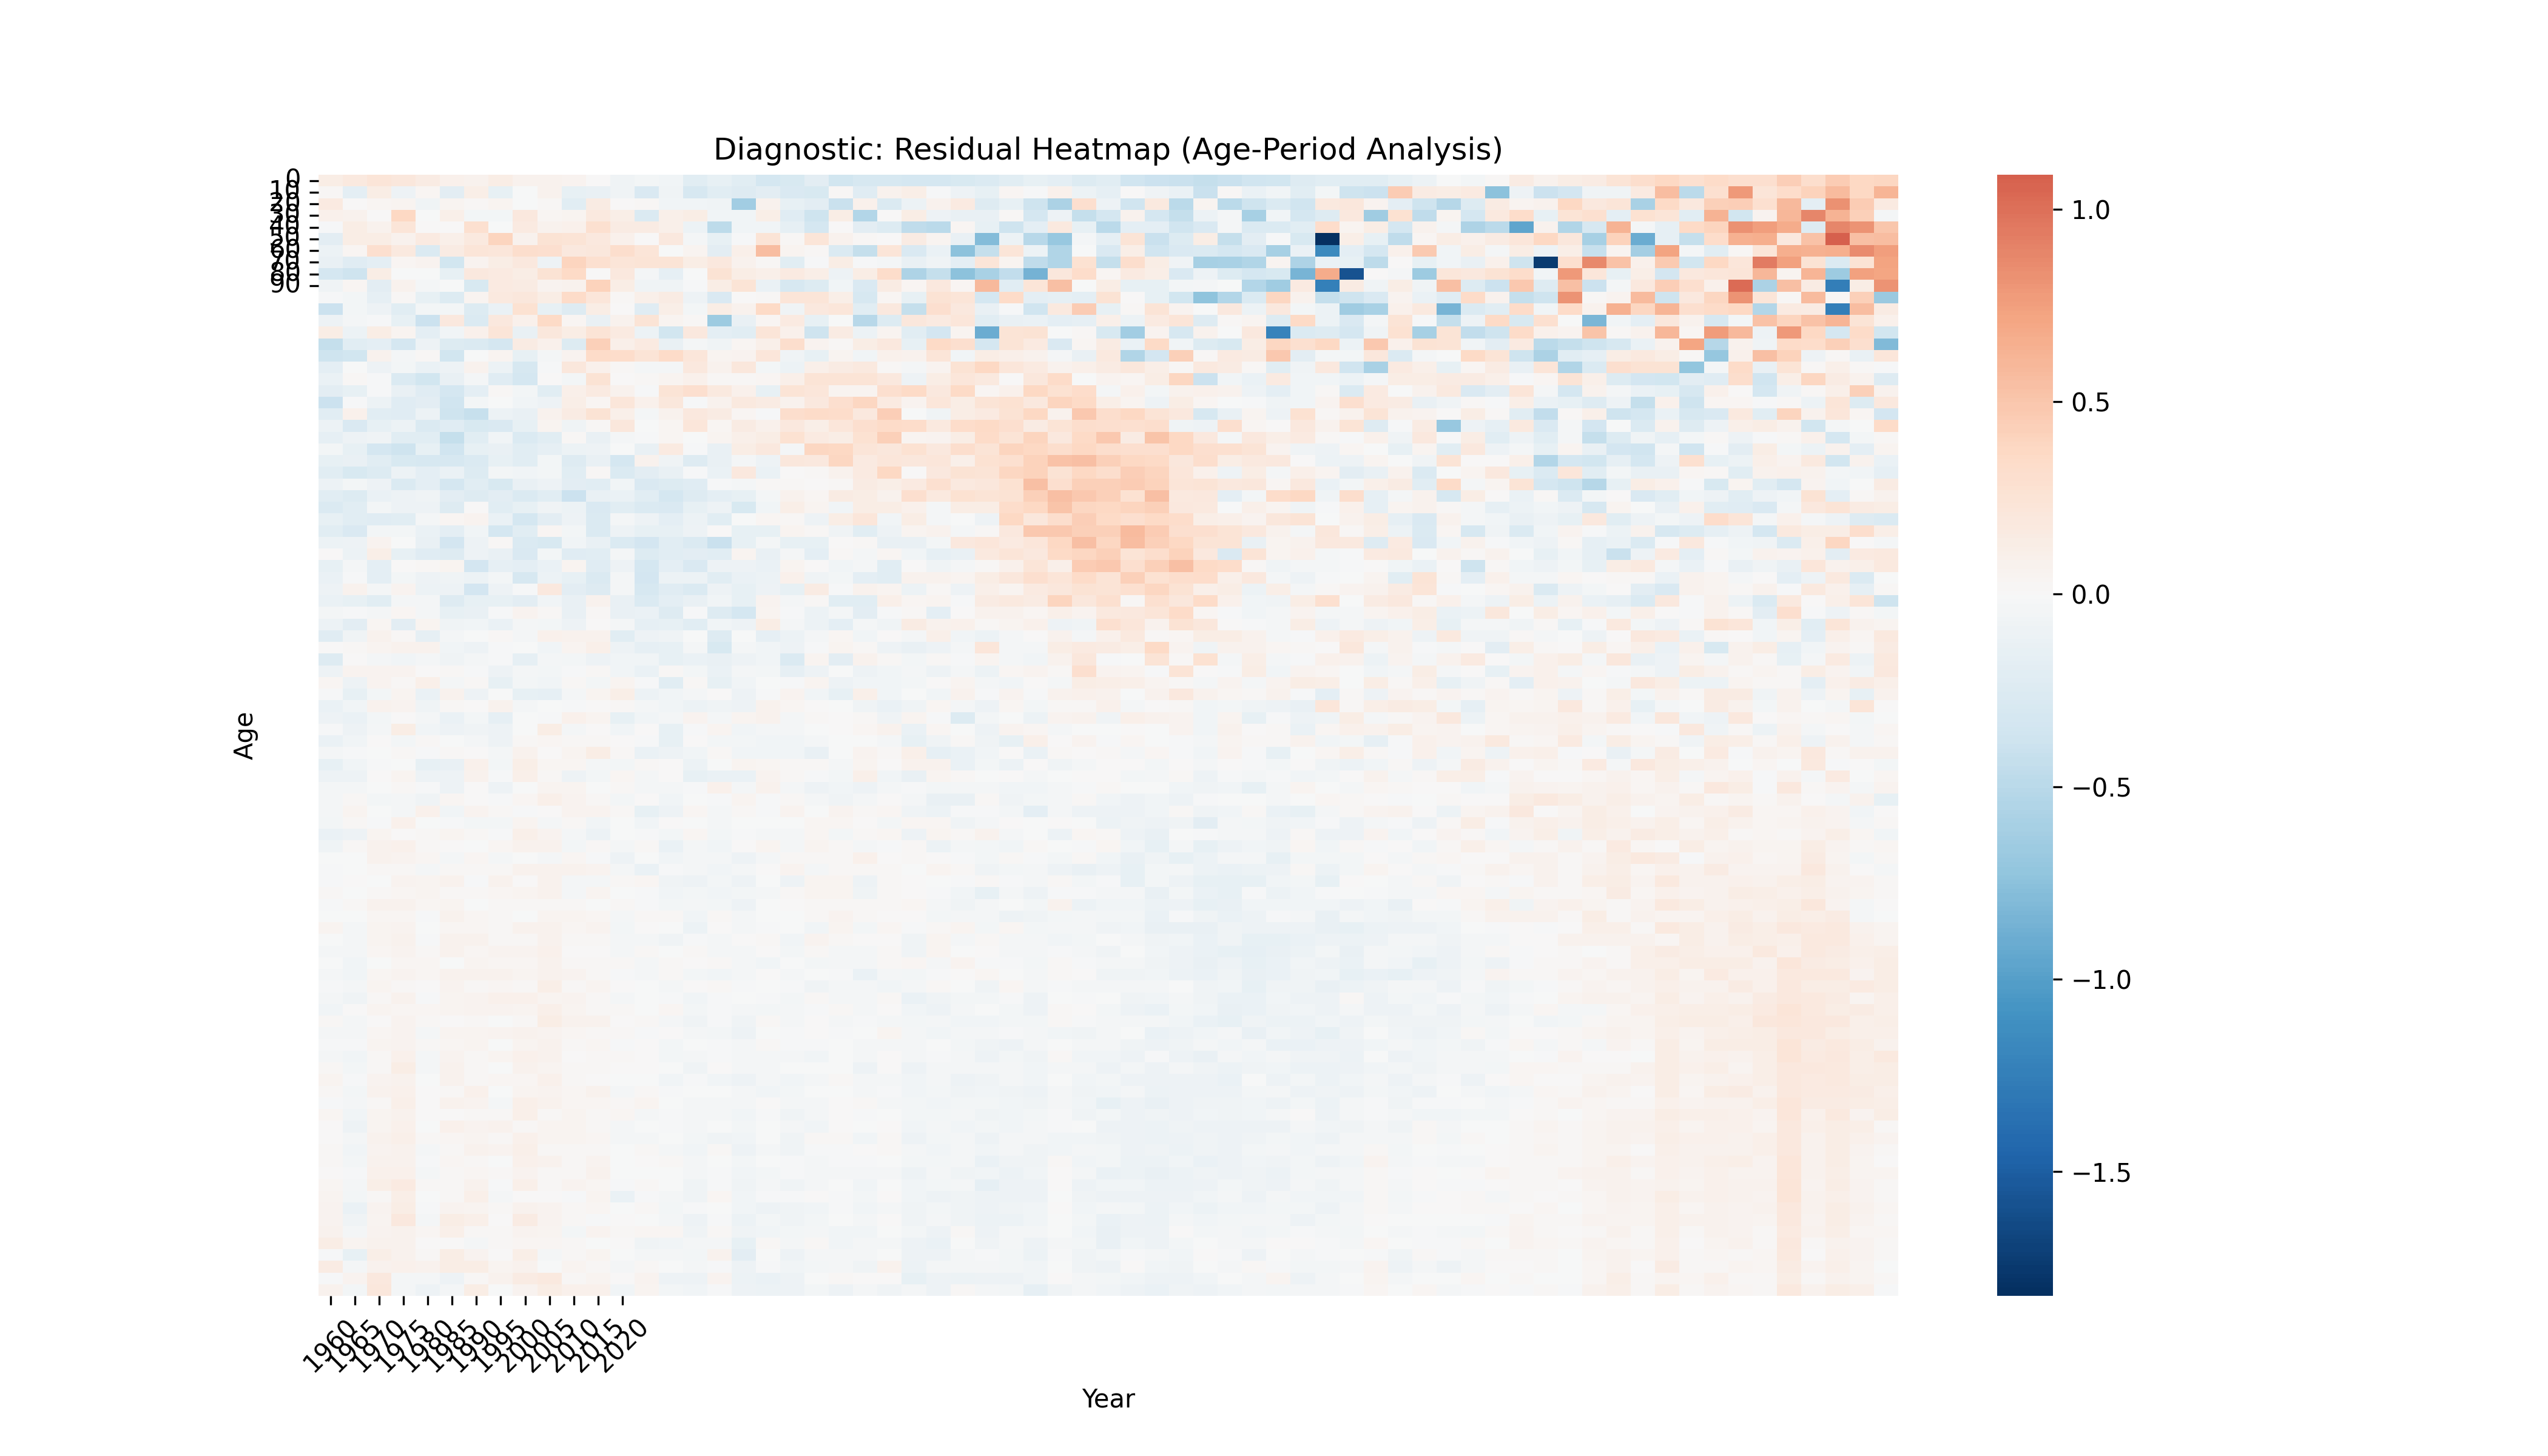
\includegraphics[width=0.9\textwidth]{figures/06_residual_heatmap_diagnostic.png}
    \caption{Diagnostic: Residual Heatmap (Age-Period Analysis). Neutral coloring indicates the absence of systematic patterns in model error.}
    \label{fig:residuals}
\end{figure}

\section{Risk Analysis and Capital Impact}

\subsection{The "Prudence Gap" and Model Risk}
The divergence in Figure \ref{fig:benchmark} represents our core finding. While Lee-Carter follows a 70-year historical linear drift, the LSTM recognizes the structural deceleration post-2010. By 2050, we identify a \textbf{38.54-point Prudence Gap}. This gap quantifies the \textbf{Model Risk}: relying on over-optimistic linear assumptions in a decelerating trend environment leads to systemic under-reserving of longevity liabilities.

\begin{figure}[h!]
    \centering
    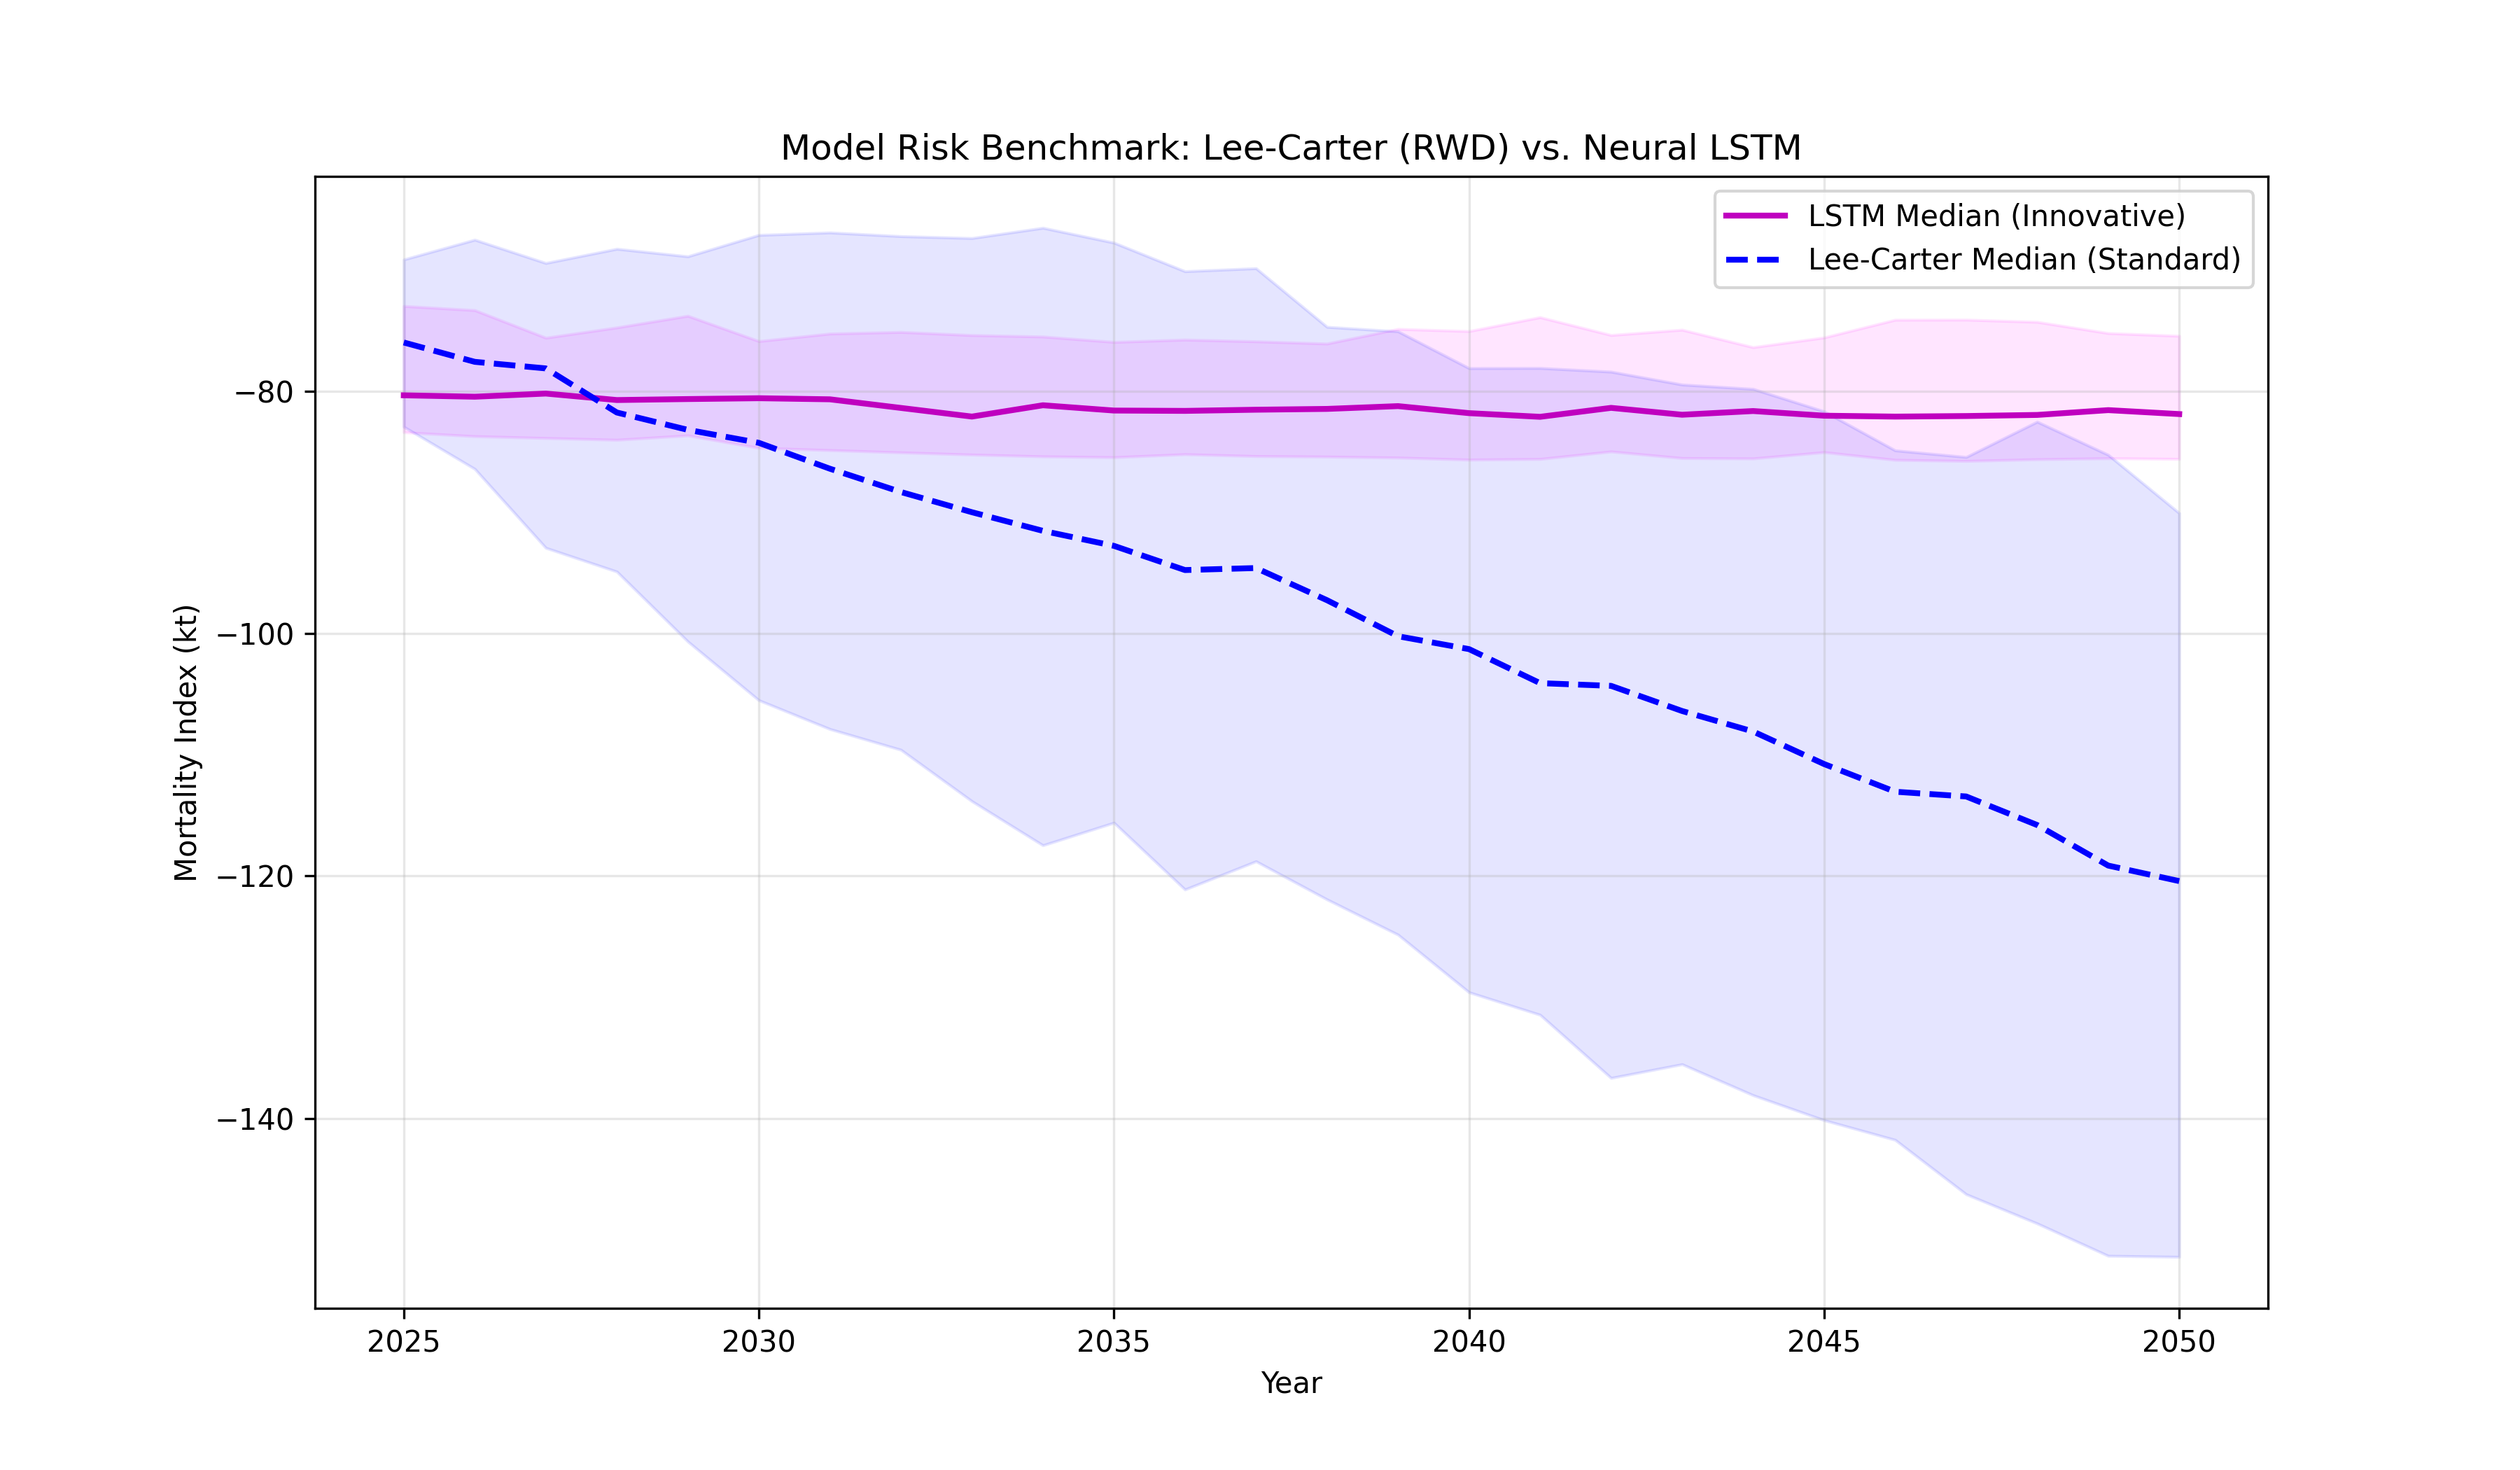
\includegraphics[width=0.9\textwidth]{figures/09_lstm_vs_lc_benchmark.png}
    \caption{Model Risk Benchmark. The divergence highlights the systemic risk of utilizing linear drift assumptions in a post-linear demographic era.}
    \label{fig:benchmark}
\end{figure}

\subsection{Expected Shortfall Calibration (SST Compliance)}
The Solvency Capital Requirement (SCR) is driven by the Expected Shortfall. We derive the longevity shock $\Delta \kt$ as:
\begin{equation}
    \Delta \kt = |\ES(\kt^{2050}) - \text{Median}(\kt^{2050})|
\end{equation}
With an $\ES$ of $-85.78$ and a median of $-81.88$, the results yield a Longevity Shock of \textbf{3.90} (Fig. \ref{fig:dist}), providing a data-driven stress scenario.

\begin{figure}[h!]
    \centering
    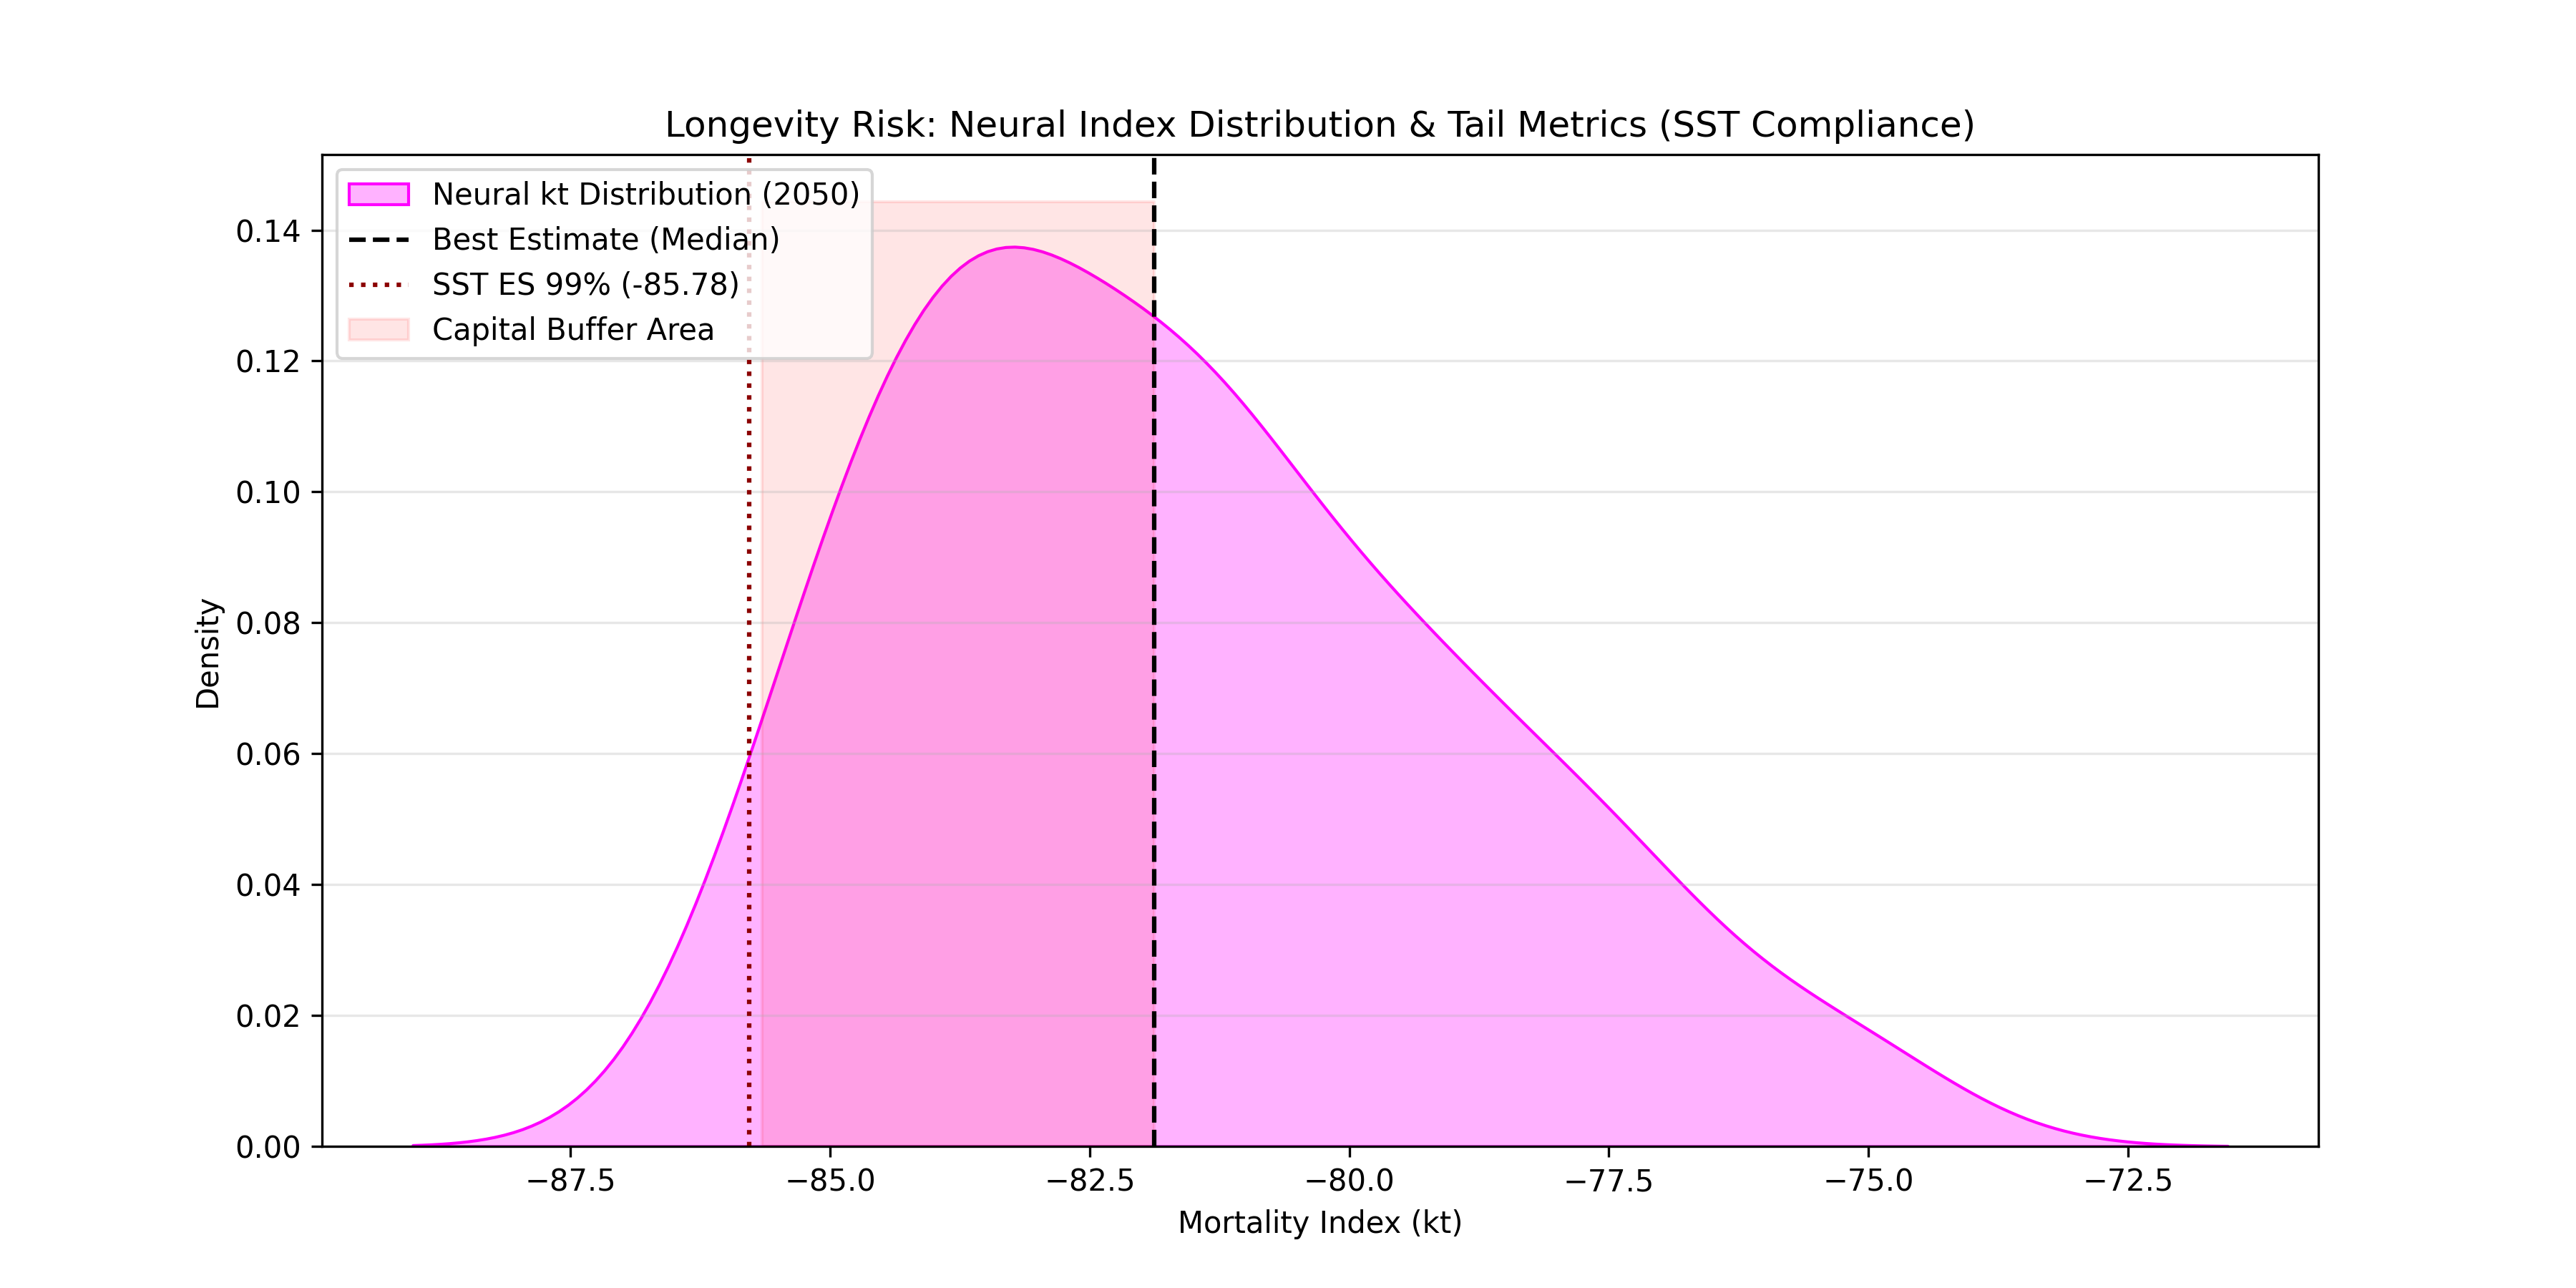
\includegraphics[width=0.9\textwidth]{figures/10_longevity_risk_distribution.png}
    \caption{Neural Index Distribution (2050). The red area represents the capital buffer required for SST compliance.}
    \label{fig:dist}
\end{figure}

\section{Conclusion and Risk Governance}
The transition to probabilistic deep learning marks a significant evolution in risk governance. Our framework offers a transparent and adaptive path for longevity modeling. By quantifying the Prudence Gap, we enable L\&H reinsurers to align technical reserves with observed demographic realities, ensuring solvency in an increasingly complex risk landscape.

\appendix
\section{Technical Appendix: Sensitivity and Robustness}
To validate the reliability of the framework for regulatory purposes, we conducted sensitivity analyses across varying look-back windows ($L \in \{5, 10, 15\}$) and hidden units ($U \in \{32, 64, 128\}$).

\subsection{Architecture Stability}
As illustrated in Figure \ref{fig:sensitivity}, the framework exhibits a performance optimum at $L=5, U=32$ (RMSE: 0.0439). While the model shows sensitivity to temporal embedding (RMSE Std Dev: 0.047), the decadal window ($L=10$) consistently outperforms the SVD baseline (RMSE: 0.1682). We utilize the $L=10, U=64$ configuration for the final calibration to maximize the epistemic uncertainty sampling capacity of the Dropout layers.

\begin{figure}[h!]
    \centering
    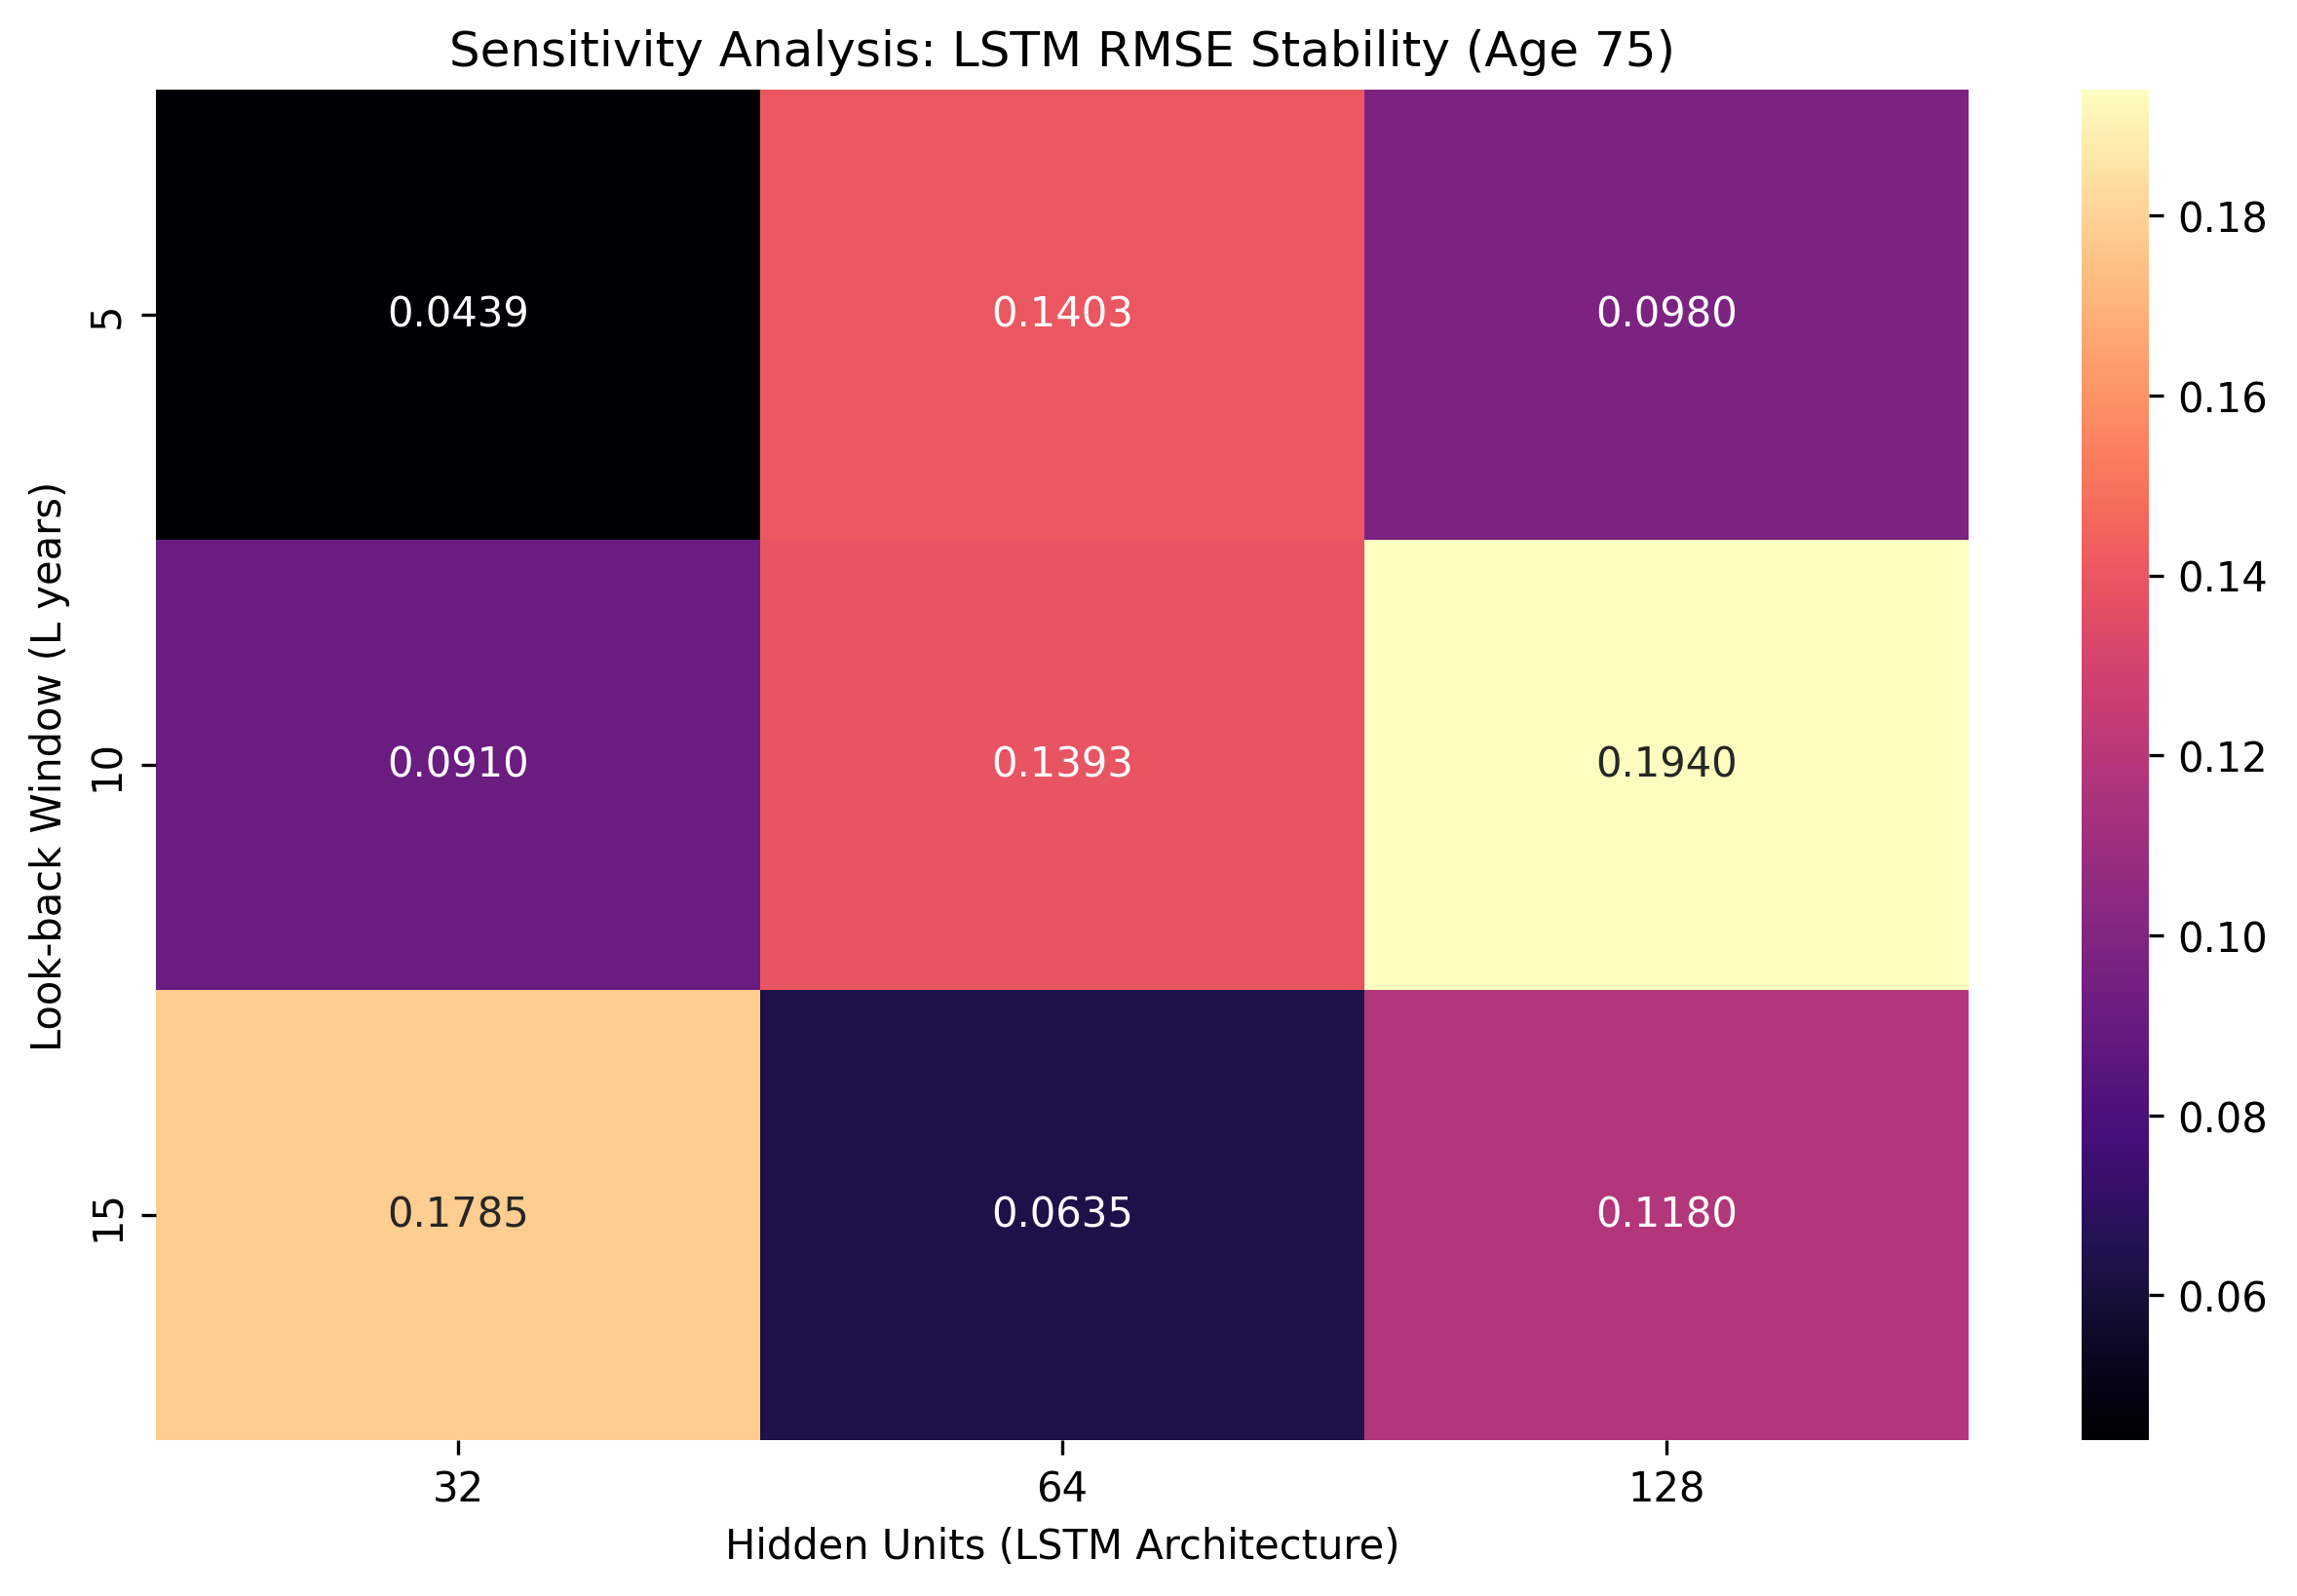
\includegraphics[width=0.8\textwidth]{figures/05_sensitivity_heatmap.png}
    \caption{Sensitivity Analysis: LSTM RMSE Stability across hyperparameters.}
    \label{fig:sensitivity}
\end{figure}

\subsection{Look-back Window Rationale}
The decadal window rationale is grounded in demographic structural changes. A 5-year window proved too sensitive to short-term volatility, while a 15-year window over-smoothed the recent deceleration signal. The 10-year configuration provides the optimal balance for capturing structural regime shifts while maintaining statistical robustness.

% --- Bibliography ---
\bibliographystyle{unsrtnat}
\bibliography{references}

\end{document}